\subsectionlink{SQUIDとその他の超伝導量子ビット}
それでは、超伝導量子二状態系、すなわち量子ビット系へ移ろう。過去10年、これらは巨視的なコヒーレンスとデコヒーレンスの実験研究で、中心的な役割を担うようになった。超伝導量子コンピューターの構成要素となる可能性も、その重要性を高めている\cite{ref274}。以下では、いわゆる超伝導量子干渉素子、略してSQUIDに焦点を当てる。Cooper対箱など、関連する他の型の超伝導量子ビット系にも触れる。

SQUIDは、さまざまな魅力的な量子効果を示せる巨視的量子系である。SQUIDでは、Bose凝縮した何十億もの電子対（以下参照）の状態が、
% 原文 p.271
\hypertarget{srcpage:271}{}\label{srcpage:271}
Schrödinger方程式に従って発展する、単一の集団的な巨視的変数で記述される。量子領域と、量子力学の限界の可能性を探索するSQUIDの潜在力は、早くから認識された。1980年、Leggett\cite{ref275}は、巨視的系で量子コヒーレントな振る舞いが可能であることを示すため、SQUIDの巨視的磁束状態の重ね合わせを含む思考実験を提案した。しかし、この提案が実験で成功するまでには、20年を要した\cite{ref276,ref277}。

\subsubsectionlink{超伝導と超電流}
超伝導現象は、1900年代初めにHeike Kamerlingh Onnesが初めて発見した。Onnesは液体Heで固体Hgを冷却し、絶対零度より数K高い温度で、Hgの電気抵抗が消えることを見いだした。1911年、「水銀の抵抗が消失する際の急激な速度について」という、適切な題名の論文\cite{ref278}で結果を公表した。2年後、この研究に対してNobel賞を授与された。しかし、微視的水準での理論的理解が得られたのは、1957年、Bardeen、Cooper、Schrieffer\cite{ref279}が、物質の結晶格子中のフォノンを介した相互引力により、逆向きのスピンを持つ電子が、いわゆるCooper対を形成することとして超伝導を説明してからであった。Cooper対は実効的にボソンとして働くため、フェルミオンである単一電子とは、著しく異なる性質を示せる。

Cooper対が、何の抵抗も受けずに物質を通過できるのは、なぜだろうか。各対は、第一励起状態からエネルギーギャップ$\Delta E$で隔てられた低エネルギー基底状態に対応することに注意しよう。結晶格子の熱振動エネルギーが$\Delta E$未満なら、格子は対の状態に遷移を誘起できず、対は格子との衝突で影響を受けない。これは、任意量のエネルギーを吸収・放出して散逸、したがって電気抵抗を生じさせる、単一の自由電子と対照的である。

超伝導の主要な特徴は、Cooper対がすべて同じ低エネルギー量子状態を取るため、多数の対が、対の集団的な重心運動を単一の巨視的波動関数で表す、無抵抗電流、すなわち「超電流」を形成できることである。量子力学の特異な特徴によって、そのような電流の流れには、外部電圧さえ必要ない。二つの超伝導物質の間に、非常に薄い絶縁障壁を入れるだけでよい。Cooper対はその障壁をトンネル通過し、電圧ゼロで超電流が流れる。この、実験的によく検証された純粋に量子力学的な現象は、いわゆるJosephson効果の、いくつかの形の一つであり、
% 原文 p.272
\hypertarget{srcpage:272}{}\label{srcpage:272}
障壁は対応してJosephson接合と呼ばれる（総説は\cite{ref280,ref281}参照）。

\subsubsectionlink{SQUIDの基本的物理}
SQUIDは、Josephson効果に直接基づく。超伝導物質の環に、一つ（rf-SQUID）または複数（dc-SQUID）のJosephson接合を入れたものである（図6.18）。本節では、単一接合のrf-SQUIDに焦点を当てる。接合を通るCooper対の量子トンネルによって、環に沿って超電流が流れ、SQUID環を貫く磁束が生じる。また、強度を調節できる外部磁場中にSQUIDを置き、追加の磁束$\Phi_{\mathrm{ext}}$を環へ与える。この外部磁束の目的は、後に説明する。

量子力学は、超電流を記述する波動関数が環に沿って連続であること、したがって波長の整数倍が環の周長に等しいことを要求する。環を一周する全位相変化は、$2\pi\Phi/\Phi_0$である。ここで$\Phi_0=h/(2e)$は、いわゆる磁束量子で、$e$は電子電荷である。$\Phi$は、超電流が作る磁束と外部磁場による$\Phi_{\mathrm{ext}}$からなる、環を貫く全捕捉磁束を表す。環にJosephson接合がなければ、波動関数の連続性は、条件
\begin{equation}\Phi/\Phi_0=k,\qquad k=1,2,\ldots\tag{6.31}\end{equation}
となる。しかしJosephson接合は、その物理的性質で完全に決まる、追加の位相シフト$\Delta\phi_{\mathrm J}$を導入する。位相連続性の完全な条件は、
\begin{equation}\Delta\phi_{\mathrm J}+2\pi\Phi/\Phi_0=2\pi k,\qquad k=1,2,\ldots .\tag{6.32}\end{equation}
\begin{figure}[htbp]\centering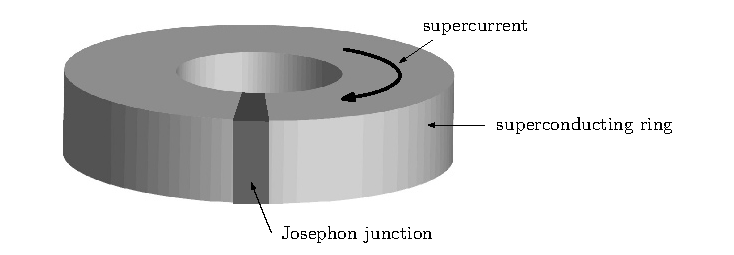
\includegraphics[width=.82\linewidth]{figures/ch06_fig18.pdf}
\caption{SQUIDの模式図。超伝導物質の環に一つまたは複数のJosephson接合を入れると、環に沿った無散逸の「超電流」が生じる。この超電流が、環を貫く磁束を作る。}
\end{figure}

% 原文 p.273
\hypertarget{srcpage:273}{}\label{srcpage:273}
$\Delta\phi_{\mathrm J}$と$\Phi_0$は固定されているので、(6.32)の唯一の自由パラメーターは全磁束$\Phi$である。したがってSQUIDでは、$10^9$個程度のCooper対という巨視的量の物質の動力学が、単一の巨視的座標$\Phi$の量子力学的発展によって、集団的に決定される。磁束が主要変数であるため、これらの素子はしばしば超伝導磁束量子ビットと呼ばれる。6.3.4節で述べるように、電荷や位相が主要変数となる、ほかの超伝導量子ビット系もある\cite{ref281}。

それでは、$\Phi$の動力学を論じよう。その発展は、次の形の有効Hamiltonianに従う。
\begin{equation}
H=\frac{P_\Phi^2}{2C}+U(\Phi)
=\frac{\hbar^2}{2C}\frac{\mathrm d^2}{\mathrm d\Phi^2}
+\left[\frac{(\Phi-\Phi_{\mathrm{ext}})^2}{2L}-\frac{I_c\Phi_0}{2\pi}\cos\left(2\pi\frac\Phi{\Phi_0}\right)\right].\tag{6.33}
\end{equation}
ここで$C$は全静電容量、$L$は環の自己インダクタンス、$I_c$はJosephson接合の臨界電流である。ここではこのHamiltonianの構造を導かない。関心のある読者は\cite{ref218}の導出を参照されたい。代わりに、それがどのような動力学を意味するのか、感覚をつかもう。

これは、ポテンシャル$U(\Phi)$中の、「質量」$C$を持つ仮想的「粒子」の運動を定めるHamiltonianと解釈できる。通常の正準変数である位置と運動量の役割は、ここでは全捕捉磁束$\Phi$と、その共役量$P_\Phi=-i\hbar\,\mathrm d/\mathrm d\Phi$が果たす。後者はしばしば全変位電流と呼ばれ、電荷の単位を持つ。実空間を動く粒子の運動エネルギーに相当するものは、ここでは静電エネルギーである。

外部磁場を調整し、誘起磁束$\Phi_{\mathrm{ext}}$をバイアス点$\Phi_{\mathrm{ext}}=\Phi_0/2$の近傍にすると、$U(\Phi)$は、傾いた一次元二重井戸ポテンシャルの形を取る（図6.19）。これが実験で関係する状況であり、以下ではこれを仮定する。傾きは$\Phi_{\mathrm{ext}}$によって決まり、$\Phi_{\mathrm{ext}}=\Phi_0/2$で、二重井戸は厳密に対称になる。この場合は後に詳しく論じる。したがって、外部印加磁場の強度で、ポテンシャルの形を変えられる。

大まかには、二つの井戸は、環を回る超電流の二方向、時計回りと反時計回りに対応する。各井戸は、接合による減衰が弱ければ、井戸間の障壁より十分低いところに局在する、Hamiltonian(6.33)のエネルギー固有状態$|k\rangle$をいくつか含む。こうして、環を回る古典的な持続時計回り電流、または反時計回り電流に、近似的に対応する、左井戸または右井戸のエネルギー固有状態の組を得る。

より正確には、波動関数$\psi_k(\Phi)\equiv\langle\Phi|k\rangle$は、局所的にs波型である。つまり、振幅は井戸の一方の底の周囲に狭いピークを持ち、
% 原文 p.274
\hypertarget{srcpage:274}{}\label{srcpage:274}
磁束空間での広がりが非常に小さい。したがって各$|k\rangle$は、全磁束$\Phi$の比較的狭い範囲に対応し、少なくとも十分小さな$k$では、磁束演算子の「ぼやけた」固有状態とみなせる。可能な離散磁束値は、連続性条件(6.32)で決まる。それゆえ$|k\rangle$は、しばしば「$k$フラクソイド状態」と呼ばれる。
\begin{figure}[htbp]\centering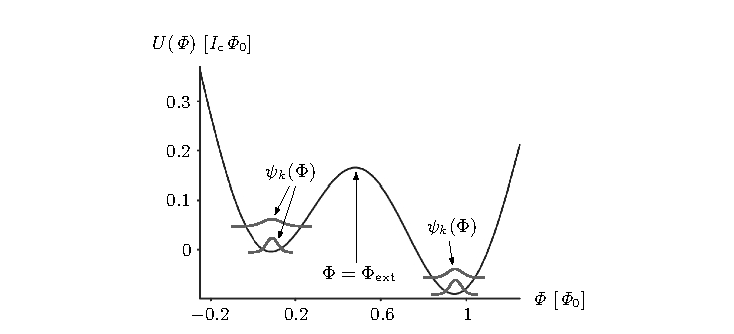
\includegraphics[width=.85\linewidth]{figures/ch06_fig19.pdf}
\caption{バイアス点$\Phi_{\mathrm{ext}}=\Phi_0/2$近傍の、SQUIDの有効二重井戸ポテンシャル$U(\Phi)$（単位$I_c\Phi_0$）。低いエネルギー固有状態$\psi_k(\Phi)\equiv\langle\Phi|k\rangle$は、各井戸の底近くによく局在し、したがって磁束演算子の近似的固有状態でもある。$\Phi$軸の単位は磁束量子$\Phi_0$で、$\Phi_{\mathrm{ext}}=3\Phi_0/5$とした。}
\end{figure}

古典的には、低い$k$フラクソイド状態$|k\rangle$のエネルギーは障壁高さ未満なので、二井戸を隔てる障壁を通過できない。しかし量子的には、井戸間の共鳴トンネルが起こり得る\cite{ref282,ref283}。たとえば放射場を加え、同じ井戸に局在する低い状態から高エネルギー状態へ系を励起すると、その状態は、その後、量子トンネルによって他方の井戸の、より低い、または等しいエネルギー準位へ減衰できる。これによって環を貫く磁束$\Phi$に巨視的変化が生じ、それが系の磁気モーメントの巨視的変化として観測できる。

通常SQUIDは、反対の井戸の底に局在する基底状態$|0\rangle$と第一励起状態$|1\rangle$が、より高い状態からエネルギー的によく分離するよう設計する。このとき、巨視的二状態系、すなわち量子ビットとして実効的に記述できる。基底には、超電流がそれぞれ確定した時計回りと反時計回りに流れる、二つの古典的持続電流状態$|\circlearrowright\rangle$、$|\circlearrowleft\rangle$を選ぶ。この二状態SQUIDの有効Hamiltonianは形式的に、
\begin{equation}\hat H=-\epsilon\hat\sigma_z-\Delta\hat\sigma_x.\tag{6.34}\end{equation}
% 原文 p.275
\hypertarget{srcpage:275}{}\label{srcpage:275}
と書ける。Pauliスピン演算子$\hat\sigma_z$の固有状態は$|\circlearrowright\rangle$、$|\circlearrowleft\rangle$であり、$2\epsilon=2I_p(\Phi_{\mathrm{ext}}-\Phi_0/2)$は、それらの非対称エネルギーを表す。$I_p\approx I_c$である。$\Delta$は二状態間のトンネル行列要素である。最低の二つのエネルギー固有状態$|0\rangle$、$|1\rangle$は、次の線形結合となる。
\begin{equation}|0\rangle=\cos\theta|\circlearrowright\rangle+\sin\theta|\circlearrowleft\rangle,\tag{6.35a}\end{equation}
\begin{equation}|1\rangle=-\sin\theta|\circlearrowright\rangle+\cos\theta|\circlearrowleft\rangle.\tag{6.35b}\end{equation}
ここで$\tan2\theta=\Delta/\epsilon$、エネルギーは$E_{0,1}=\mp\sqrt{\Delta^2+\epsilon^2}$である。したがって、$|0\rangle$と$|1\rangle$のエネルギー分裂は、$\Delta E=2E_1=2\sqrt{\Delta^2+\epsilon^2}$となる。バイアス点$\Phi_{\mathrm{ext}}=\Phi_0/2$から離れると、$\epsilon\gg\Delta$であり、$|\circlearrowright\rangle$、$|\circlearrowleft\rangle$は、それぞれゼロフラクソイド、1フラクソイドのエネルギー固有状態$|0\rangle$、$|1\rangle$と本質的に同一となる。これは上の議論に一致する。二状態$|0\rangle$、$|1\rangle$に対応する超電流の期待値は、$\pm I_p\cos2\theta$となることを示せる。正符号は時計回りを表す。

\subsubsectionlink{SQUIDの重ね合わせ状態とコヒーレント振動}
SQUIDがバイアス点$\Phi_{\mathrm{ext}}=\Phi_0/2$にあると何が起こるかを考えよう。二重井戸は対称になり、(6.34)で$\epsilon=0$となる。すなわち、左右の井戸のエネルギー準位がそろう。この場合、古典的には$|0\rangle$と$|1\rangle$の準位が交差し、縮退する。しかし量子的には、井戸間のトンネル障壁$\Delta$［(6.34)参照］が存続することで縮退が解ける。これが準位の「反発」をもたらし、反交差を生む（図6.20）。(6.35a)、(6.35b)では$\theta=\pi/4$なので、基底状態と第一励起状態は、持続電流状態の対称・反対称重ね合わせとなる。
\begin{equation}|0\rangle=\frac1{\sqrt2}(|\circlearrowright\rangle+|\circlearrowleft\rangle),\tag{6.36a}\end{equation}
\begin{equation}|1\rangle=\frac1{\sqrt2}(-|\circlearrowright\rangle+|\circlearrowleft\rangle).\tag{6.36b}\end{equation}
二つの新しい固有状態のエネルギー分裂$\Delta E$は、通常非常に小さく、接合の静電容量$C$だけで決まり、$\Delta E\propto e^{-\sqrt C}$とスケールする。

$|\circlearrowright\rangle$と$|\circlearrowleft\rangle$はそれぞれ左右の井戸に局在するので、重ね合わせ(6.36a)、(6.36b)は、二井戸にわたって非局在化している。この存在は、2000年、Friedmanら\cite{ref276}と、独立にvan der Walら\cite{ref277}が実験で確認した。Friedmanらの実験では、二状態はそれぞれ、何十億ものCooper対からなる、数$\mu\mathrm A$の逆方向の超電流に対応した。
% 原文 p.276
\hypertarget{srcpage:276}{}\label{srcpage:276}
これは、二電流の作る磁束に$\Phi_0/4$以上の巨視的差があることに当たり、局所磁気モーメントでは約$10^{10}\mu_{\mathrm B}$に等しい。$\mu_{\mathrm B}$はBohr磁子である。ゆえに、(6.36a)、(6.36b)は、20年前のLeggettの思考実験\cite{ref275}が描いたとおりの、巨視的に異なる状態のSchrödingerの猫型重ね合わせを表す。Friedmanらは、二状態間のエネルギー差$\Delta E$の静的分光測定という間接的方法で、存在を検証した。得られた$\Delta E$は、理論予測と極めてよく一致した。
\begin{figure}[htbp]\centering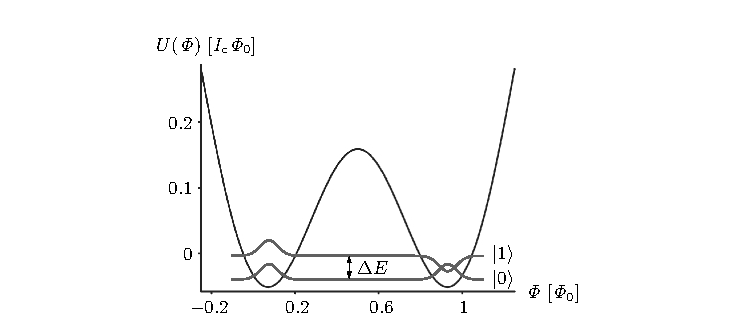
\includegraphics[width=.85\linewidth]{figures/ch06_fig20.pdf}
\caption{バイアス$\Phi_{\mathrm{ext}}=\Phi_0/2$でのSQUIDの有効ポテンシャル。この点で二重井戸は対称になる。トンネル障壁が井戸の準位交差を妨げ、非局在化した固有状態$|0\rangle=(|\circlearrowright\rangle+|\circlearrowleft\rangle)/\sqrt2$（新しい対称基底状態）、$|1\rangle=(-|\circlearrowright\rangle+|\circlearrowleft\rangle)/\sqrt2$（新しい反対称第一励起状態）の形成を介して、反交差が起こる。これらは「古典的」持続電流状態の重ね合わせである。存在は、分光測定\cite{ref276,ref277}とコヒーレントRabi振動の観測\cite{ref284,ref285}によって、実験的に確認された。}
\end{figure}

そのような重ね合わせの存在を示す別の方法は、持続電流状態間のコヒーレント振動を観測することである。これは6.1.1節のRabi型振動である。まず、SQUIDを貫く外部磁束を、縮退点$\Phi_{\mathrm{ext}}=\Phi_0/2$からわずかにずらし、エネルギー固有状態$|0\rangle$と$|1\rangle$を縮退近くにする。緩和させることで基底状態$|0\rangle$に初期化する。次に、二状態間の小さなエネルギー差$\Delta E$に周波数を合わせた、マイクロ波パルスを加える。Rabi振動の議論によれば、量子ビットは$|0\rangle$と$|1\rangle$の間、したがって持続電流状態間でも振動する［(6.35)参照］。
% 原文 p.277
\hypertarget{srcpage:277}{}\label{srcpage:277}
これは、巨視的超電流が環の時計回りと反時計回りの間で振動することとして現れる（図6.21）。振動はRabi周波数で起き、その周波数は量子ビットとマイクロ波場の結合強度で決まり、マイクロ波振幅に線形に依存する。したがって、SQUIDが二状態の各々にある相対確率は、パルスの振幅と長さに依存する［(6.8)参照］。

2003年、Chiorescuたち\cite{ref284}は、超伝導磁束量子ビットでこのRabi振動を実験的に示した。実験系は、三つのJosephson接合を入れた、$\mu\mathrm m$サイズの超伝導環からなる（図6.22）。単一接合のrf-SQUIDに比べ、三接合を使っても基本物理は大きく変わらないが、適切な調整が容易になる。量子ビットはさらに、Josephson接合を二つ持つdc-SQUIDに結合され、それが量子ビットの磁束を読む極めて高感度な装置として働く。

Chiorescuらは、与えられた長さと振幅のマイクロ波パルスを加え、次に、実験で利用できる観測量に対応する、持続電流基底$\{|\circlearrowright\rangle,|\circlearrowleft\rangle\}$で射影測定を行った。
\begin{figure}[htbp]\centering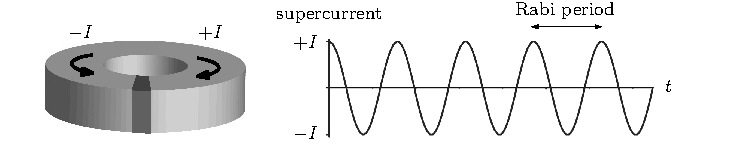
\includegraphics[width=.9\linewidth]{figures/ch06_fig21.pdf}
\caption{縮退点$\Phi_{\mathrm{ext}}=\Phi_0/2$の近くに調整したSQUIDの量子コヒーレントなトンネルは、巨視的超電流が時計回りと反時計回りの間でコヒーレントに振動することによって観測できる。}
\end{figure}
\begin{figure}[htbp]\centering
\includegraphics[width=.9\linewidth]{figures/ch06_fig22.pdf}
\caption{Chiorescuら\cite{ref284}の実験に使われた超伝導磁束量子ビット。右側の実際の量子ビットは、三つのJosephson接合を持つ小さな超伝導環である。白黒の矢印は持続電流の二方向を示す。量子ビットと一部を共有する、より大きい超伝導環に二接合を入れたSQUIDが、磁束の変化を検出する。許可を得て\cite{ref284}から転載。Copyright 2003 by AAAS.}
\end{figure}
% 原文 p.278
\hypertarget{srcpage:278}{}\label{srcpage:278}
この手順を数千回行い、たとえば超電流が時計回りとなる$|\circlearrowright\rangle$状態に、量子ビットを見いだす実験的確率を得た。マイクロ波振幅を固定し、パルス長を変えて繰り返すと、約150nsという驚くほど長い減衰時間を持つ、数百回の減衰Rabi振動を追跡できた（図6.23）。それが実際にRabi型の量子コヒーレント振動であると確認するため、研究者たちは、観測された周波数がマイクロ波振幅に線形比例することを検証した。これはRabi過程の主要な特徴である。別の連続読出し方式は、その後のIlichevら\cite{ref285}の実験で実現された。

Chiorescuら\cite{ref284}とIlichevら\cite{ref285}のRabi振動は、以前のFriedmanら\cite{ref276}とvan der Walら\cite{ref277}の分光結果とともに、巨視的に異なる超電流状態のコヒーレントな重ね合わせの存在を、印象的に示す。
\begin{figure}[htbp]\centering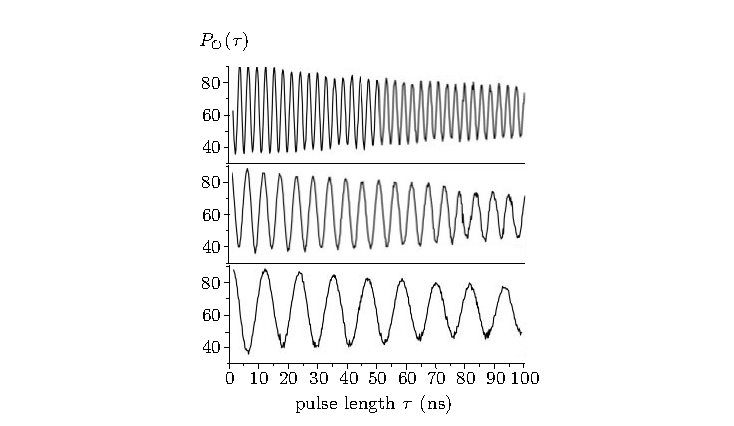
\includegraphics[width=.8\linewidth]{figures/ch06_fig23.pdf}
\caption{Chiorescuら\cite{ref284}の実験で観測された、超伝導磁束量子ビットの巨視的な逆方向超電流状態$|\circlearrowright\rangle$と$|\circlearrowleft\rangle$の間のRabi振動。これは二状態のコヒーレント重ね合わせを確認する。共鳴マイクロ波の三つの振幅の結果を示し、上から下へ振幅が小さくなる。縦軸は、特定の確定電流状態、たとえば$|\circlearrowright\rangle$に見いだされた実験の割合$P_{\circlearrowright}(\tau)$（\%）を、パルス長$\tau$の関数として示す。許可を得て\cite{ref284}の図を改作。Copyright 2003 by AAAS.}
\end{figure}
% 原文 p.279
\hypertarget{srcpage:279}{}\label{srcpage:279}
SQUIDは、この種の重ね合わせ状態の生成に特に適している。SQUID環を貫く捕捉磁束という、関係する巨視的変数を、Josephson接合の微視的なエネルギー差で制御できるからである\cite{ref286}。トンネル障壁の高さ$\Delta$は、環の大きさとは独立に、主として接合の性質で決まる。これは、達成可能な巨視的磁束状態の重ね合わせの「大きさ」が、異なりの程度そのもの、すなわち持続電流状態間の磁束差に、弱くしか依存しないことを意味する。

この特徴によって、ほかの実験で達成したものよりも、巨視的な異なりの程度がはるかに大きい「古典的」状態の重ね合わせを作れる。たとえば$\mathrm C_{70}$分子の物質波回折実験（6.2節）では、回折模様を観測するため、分子中の原子数$N$に伴って、回折格子の間隔を$1/\sqrt N$に従って減らす必要がある。したがって、この場合、ある大きさの分子の干渉模様を実験で作る能力は、分子の大きさ自体に応じて変わる。

\subsubsectionlink{デコヒーレンスを観測し定量化する}
振動する占有確率の包絡線の減衰（図6.23参照）から導かれる、Rabi振動の特徴的減衰時間は、持続電流重ね合わせ(6.36a)、(6.36b)に固有のデコヒーレンス時間尺度を、直ちに与えるわけではないことに注意が必要である。Rabi振動は、加えたマイクロ波パルスという外部駆動場によって誘起されるためである。しかしデコヒーレンス時間を測るには、制御されない環境と相互作用する量子ビットが、自由に、すなわち駆動なしで発展する間に、重ね合わせ成分間の相対位相情報が非局在化することを考えなければならない。

この目標は、Ramsey干渉法\cite{ref051}で達成できる。以下の手順は、2.2.2節で述べた「共鳴」Ramsey法の変形である。まず、量子ビットを縮退点$\Phi_{\mathrm{ext}}=\Phi_0/2$近くに設定し、再びエネルギー基底状態$|0\rangle$に初期化する。次に、二準位間の遷移周波数$\Delta E/(2\pi)$から$\delta f$だけ離調した、$\pi/2$マイクロ波パルスを加える。これにより$|0\rangle$と$|1\rangle$のコヒーレント重ね合わせへ変換し、時間$\tau$だけ自由に発展させる。この間、加えたマイクロ波周波数で回転する座標系では、相対位相が$2\pi(\delta f)\tau$だけ増す。その後、第二の非共鳴$\pi/2$パルスを加える。得られる重ね合わせでは、$|0\rangle$と$|1\rangle$の係数の大きさが、周波数$\delta f/2$で、遅延時間$\tau$に振動的に依存する。したがって、古典的な持続電流状態の占有確率は、
% 原文 p.280
\hypertarget{srcpage:280}{}\label{srcpage:280}
周波数$\delta f$で、$\tau$の関数として振動する。

実際には、量子ビットの自由発展時間$\tau$の間に、デコヒーレンスが二つのエネルギー状態、したがって持続電流状態間のコヒーレンスを減らすので、振動振幅は減衰すると予想する。2.2.2節で説明したように、完全にデコヒーレンスすると、占有確率が$\tau$に依存しない、持続電流状態の非コヒーレント混合へ至る。

遅延時間を増すと占有確率の振動がやがて消えることにより、デコヒーレンスの漸進的効果を観測し、定量化できる。Chiorescuら\cite{ref284}は、さまざまな遅延時間で、持続電流状態の関係する占有確率を測った。その減衰振動を追い、特徴的デコヒーレンス時間尺度を読み取った（図6.24）。

予想された、遅延時間への振動的依存性が見られる。振動周波数はマイクロ波の離調$\delta f$に一致し、Ramsey理論の予測と極めてよく一致した。包絡線の減衰から約20nsのデコヒーレンス時間を得た。これは、この実験で量子ビットが自由発展する間に、古典的な持続電流状態間の位相コヒーレンスが、環境によって失われる特徴的時間尺度である。

より最近の磁束量子ビット実験では、最大$4\,\mu\mathrm s$という、はるかに長いデコヒーレンス時間が観測された\cite{ref287}。この有望な結果は、超伝導量子ビットが固体量子計算素子の実現に適するかもしれないという期待を高めた（第7章参照）。制御パルスによるゲート操作は非常に速く、単一量子ビットゲート操作は約2nsで行える。
\begin{figure}[htbp]\centering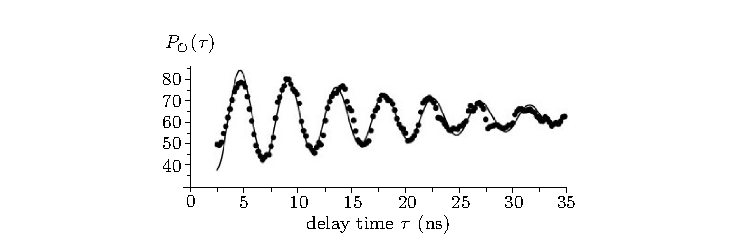
\includegraphics[width=.85\linewidth]{figures/ch06_fig24.pdf}
\caption{Chiorescuら\cite{ref284}の実験で観測された、超伝導磁束量子ビットへの二つの$\pi/2$パルスの遅延時間$\tau$に対する、占有確率$P_{\circlearrowright}(\tau)$の依存性。振動振幅の減衰は、系からの漸進的なコヒーレンスの喪失に対応する。許可を得て\cite{ref284}の図を改作。Copyright 2003 by AAAS.}
\end{figure}
% 原文 p.281
\hypertarget{srcpage:281}{}\label{srcpage:281}
したがって、コヒーレンスを相当失うまでに、1000回程度のゲート操作が可能かもしれない。しかし、単純な量子アルゴリズムにも必要な$O(100{,}000)$回には、まだかなり遠い。

SQUIDの磁束変数の代わりに、電荷または位相を主要変数とする超伝導素子でも、量子コヒーレント振動とデコヒーレンスが観測されている。一般に、超伝導電荷・位相素子の物理の形式的記述は、上述のSQUIDとよく似ている。

一般にCooper対箱として知られる超伝導電荷量子ビットは、貯蔵庫からJosephson接合を通ってCooper対がトンネルできる、小さな超伝導「島」からなる。二つの量子ビット基底は、少なくとも一つのCooper対だけ異なる、島の二つの電荷状態に対応する。Cooper対箱は、電荷状態間のRabi振動を実験観測できた、最初の超伝導量子ビット系であり、1999年にNakamura、Pashkin、Tsai\cite{ref288}が達成した。2002年にはVionら\cite{ref289}が、$0.5\,\mu\mathrm s$のデコヒーレンス時間を持つ、数千回のコヒーレント振動を報告した。

Rabi型のコヒーレント振動は、位相量子ビットでも観測された。位相量子ビットはrf-SQUIDと同様、単一のJosephson接合を含む。ただし、環を貫く磁束の代わりに、主要変数は接合電極間の位相差である。Yuら\cite{ref290}は、巨視的に異なる位相状態間のRabi振動を測り、最大数$\mu\mathrm s$のデコヒーレンス時間を得た。Martinisら\cite{ref291}も、同様の結果を報告した。

現在の実験的証拠（たとえば\cite{ref291,ref292}参照）は、超伝導量子ビットのデコヒーレンスの主な源が、予想されそうな、環・接合系を制御する外部回路との相互作用ではなく、Josephson接合と超伝導体の内部欠陥の存在であることを示す。これらの欠陥は、しばしば有効二準位系として模型化できる。5.1.2節で触れたように、超伝導系などの低温系のデコヒーレンスと散逸が、主にこのような内部二準位系によることは、しばらく前から知られている\cite{ref199,ref200}。量子ビット自体が二準位系なので、そのデコヒーレンスの理論的記述に適切な模型は、5.4節のスピン・スピン型である可能性が高い\cite{ref199}。

たとえばMartinisら\cite{ref292}は、絶縁体のバルクとJosephson接合の両方にある二準位状態による誘電損失が生む、超伝導位相量子ビットのデコヒーレンス研究へ、この模型を適用した。理論研究から得た知見は、著しく改善された実験構造へ、成功裏に反映された。ほかの理論研究は、電流バイアスJosephson接合を制御するバイアス電流の揺らぎなど、雑音過程の影響を調べている\cite{ref293}。しかし、
% 原文 p.282
\hypertarget{srcpage:282}{}\label{srcpage:282}
2.12節の一般的議論（7.3節も参照）に照らすと、そのような雑音による集団の位相緩和と、環境とのもつれが生む「真の」デコヒーレンスを、明瞭に区別することが重要である。局所測定統計という現象論的視点では、両者が同様の結果を生むとしても、同じではない。
\subsectionlink{その他の実験領域}
前の各節では、中間的尺度および巨視的尺度で異なる状態の重ね合わせを生成・検出し、その漸進的デコヒーレンスを観測できた実験を述べた。これらでは、実験室で観測された量子から古典への現象を、デコヒーレンスが定性的・定量的に説明した。

同じように、ただし別の視点から、ある実験で重ね合わせ状態を生成・観測できない原因を理解するうえでも、デコヒーレンスは役立つ。本節では、現在までに得られたものよりも、さらに大きい非古典的重ね合わせを、将来生成・観測するための有望な候補となる、二つの実験領域を述べる。見るように、それらで重ね合わせの生成・観測がこれほど難しい理由を、デコヒーレンスによって定性的・定量的に記述できる。また、実験手順の改善方法を示唆し、実験室で望ましい重ね合わせを作る目標に、さらに近づくことも可能にする。

\subsubsectionlink{Bose--Einstein凝縮体におけるデコヒーレンス}
Bose--Einstein凝縮は、巨視的数の原子が、ある実験では最大$O(10^7)$個まで、量子相転移を起こし、すべての原子が個別性を失って同一量子状態を占める凝縮体となる、量子力学的現象である。したがって凝縮体は、位相を持つ単一の量子力学的$N$粒子波動関数で完全に記述できる。この位相は実験で調べられる。たとえば二つの凝縮体を重ねると、両者の位相差による干渉模様が観測される\cite{ref294,ref296,ref297,ref298,ref299}（図6.25）。最近は、単一凝縮体をコヒーレントに分割し、その後再結合して干渉縞を観測する干渉計も作れるようになった\cite{ref295}（同じく図6.25参照）。

このような量子的性質の実証の成功にもかかわらず、粒子数が巨視的に区別される状態の重ね合わせに、凝縮体を準備する実験は、いくつかの有望な理論提案\cite{ref300,ref301,ref302,ref303,ref304,ref305,ref306}があるにもかかわらず、これまで失敗している。
% 原文 p.283
\hypertarget{srcpage:283}{}\label{srcpage:283}
しかし、関係するデコヒーレンス機構を考慮すれば、この失敗は定性的にも定量的にもよく理解できる。凝縮体の重ね合わせ状態では、デコヒーレンスは主に、凝縮原子と非凝縮原子の間の、弾性・非弾性散乱によることが分かる。
\begin{figure}[htbp]\centering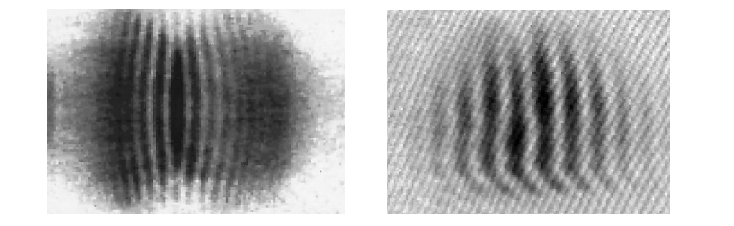
\includegraphics[width=.94\linewidth]{figures/ch06_fig25.pdf}
\caption{Bose--Einstein凝縮体の原子気体密度の干渉模様。左：独立な二凝縮体を重ねたときの、位相差による模様。許可を得て\cite{ref294}から転載。Copyright 1997 by AAAS. 右：凝縮体の「二重スリット」干渉計で得られた干渉縞。単一凝縮体をコヒーレントに分割し、通常の二重スリットの役割を模擬した後、再結合した。許可を得て\cite{ref295}から転載。Copyright 2004 by the American Physical Society.}
\end{figure}

この散乱過程の詳細な模型が作られ（たとえば\cite{ref102}参照）、凝縮体の大きさなどの主要実験パラメーターの関数として、デコヒーレンス時間尺度の現実的予測が得られる。また、これらの模型の知見は、巧妙な実験設計によってデコヒーレンスを最小にする具体的提案を生んだ。改善案には、デコヒーレンスを誘起する非凝縮原子の熱的雲を、より速く蒸発させる、修正した凝縮体トラップ\cite{ref102}、粒子数差状態ではなく相対位相状態の巨視的重ね合わせを作り、環境の選ぶ指針基底を考慮してデコヒーレンスを最小にすること\cite{ref303}、熱的雲の実効的大きさを減らす能動的な環境設計（7.5.3節）\cite{ref102}、重ね合わせ状態のより速い生成\cite{ref306}などがある。各提案は、特定の実験配置に関係する、さまざまなデコヒーレンス機構の分析から導かれる。配置が与えられると、模型は量子・古典境界の位置と、望ましい猫状態を実現するため、その境界を押し進めるには何ができ、何をすべきかを教える。

% 原文 p.284
\hypertarget{srcpage:284}{}\label{srcpage:284}
\subsubsectionlink{量子電気機械系におけるデコヒーレンス}
量子電気機械系、略してQEMSは、さらに大きい非古典的重ね合わせを生成する可能性を持つ、多彩な実験の仲間に、比較的最近加わったものである\cite{ref307}（入門は\cite{ref308,ref309}も参照）。QEMSには、デコヒーレンスと散逸の「振動子・スピン模型」との関連で、5.4.2節ですでに触れた。何十億もの原子が、空間中のよく区別できる二位置の重ね合わせにある、真に機械的な「Schrödingerの子猫」を示すために、QEMSは非常に有望である。この分野の急速な実験進展から、今後数年で、量子から古典への移行の探索で中心的な役割を果たす可能性が高い。

QEMSは、近年のナノテクノロジーの革命の成果である。主要部分は、シリコンなどの結晶材料から作る、小型の両端固定梁または片持ち梁で、典型寸法はnmから$\mu\mathrm m$程度である（図6.26）。梁は小さな機械的共振器として働く。短時間適切な駆動力を加えると、振動運動を始める。

寸法が極めて小さいため、機械系であることを考えると、振動周波数は驚くほど高くできる。最近の実験では、マイクロ波領域の1GHzまで達成した\cite{ref311}。また、共振器の散逸は比較的弱くでき、振幅が有意に減少するまでに、数万回自由振動する。運動は電子トランスデューサーで検出し、対応する電気信号へ変換して読み出す。
\begin{figure}[htbp]\centering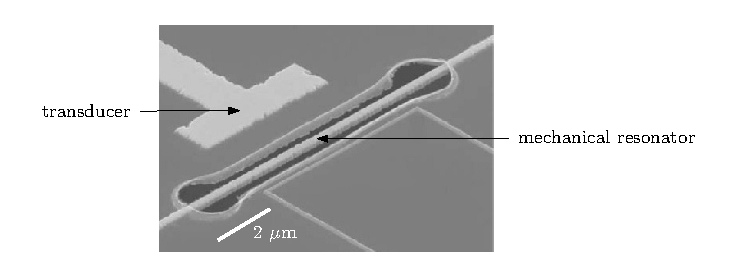
\includegraphics[width=.94\linewidth]{figures/ch06_fig26.pdf}
\caption{Cornell UniversityのKeith Schwabの研究室\cite{ref310}で作られた、量子電気機械系の実験的実現。幅200nm、長さ$8\,\mu\mathrm m$の梁が、固有周波数19.7MHzのナノ機械共振器として働く。電子トランスデューサーで、梁の振動を電気信号へ変換する。許可を得て\cite{ref310}から転載。Copyright 2004 by AAAS.}
\end{figure}
% 原文 p.285
\hypertarget{srcpage:285}{}\label{srcpage:285}
注目すべきことに、共振器の大部分の自由度は、QEMSの典型的動作温度であるmKという低温で「凍結」されるか、トランスデューサーへの結合が無視できる。したがって多くの場合、巨視的共振器は、梁の最低の基本曲げモードに対応する、単一の量子力学的調和振動子として実効的に扱える。QEMSのナノ機械共振器は、何十億もの原子からなり、多数の内部欠陥や不完全さで乱された、巨視的機械物体である。それにもかかわらず、これから述べるように、明確に量子力学的な効果を示せる。

QEMSの主要な特徴は、空間変位への極めて高い感度である。重要な量は、位置検出の量子限界を表す、調和振動子の量子零点変位の不確定性$\Delta x_{\mathrm{zp}}$である。現在実験室で作られるナノ機械共振器では、わずか0.1pm程度である\cite{ref307}。それでも最近の実験では、たとえば図6.26のQEMSを用い、$\Delta x_{\mathrm{zp}}$の数倍に至るまで空間変位を分解できた\cite{ref310}。したがって、量子限界での位置測定という目標に非常に近づいている。

\subsubsectionlink*{QEMSによる機械的「Schrödingerの子猫」の生成法}
研究者たちは、共振器を二つの異なる空間変位のコヒーレント重ね合わせに置き、その漸進的デコヒーレンスを観測する可能性も考えている。特に面白いのは、QEMSが、たとえば超伝導量子ビット（6.3節）やBose--Einstein凝縮体（6.4.1節）よりも、日常世界の物体にはるかに近い、純粋な機械構造であることだ。実現すれば、それは、巨視的で「粗い」通常物質の機械物体が、二つの異なる位置にある重ね合わせを表す。現時点では、そのような重ね合わせはまだ実験室で実現されていないが、具体的提案\cite{ref312}があり、関係するデコヒーレンス・散逸機構の理論研究も進んでいる\cite{ref242,ref313,ref314,ref315}。巨視的距離だけ離れた複数の共振器をもつれさせる考えも、理論的に調べられた\cite{ref316}。量子コンピューターの機械的量子ビットとして使う可能性も、考えられる\cite{ref317}。

Armour、Blencowe、Schwab\cite{ref312}の提案した、QEMSの空間的重ね合わせの生成法を簡単に概説しよう（\cite{ref307}も参照）。基本的考えは、基底状態$|0\rangle$、$|1\rangle$が共振器の異なる二変位へ結合し、しかもそれらの重ね合わせへ比較的容易に準備できる、二状態量子系を使うことである。
% 原文 p.286
\hypertarget{srcpage:286}{}\label{srcpage:286}
\cite{ref312}ではCooper対箱を選んだ（6.3.4節参照）。二基底状態は、超伝導島上の異なる電荷値に対応する。箱と片持ち梁の静電相互作用は、箱が$|0\rangle$か$|1\rangle$かに応じて、共振器に二つの異なる変位を与える（図6.27）。対応する重心位置状態を、$|P_0\rangle$、$|P_1\rangle$と書こう。

箱を$(|0\rangle+|1\rangle)/\sqrt2$の重ね合わせに準備する。\cite{ref312}が示したように、特定の制御パルス列を箱へ加えると、もつれた箱・共振器の重ね合わせ
\begin{equation}|\Psi\rangle=\frac1{\sqrt2}(|0\rangle|P_0\rangle+|1\rangle|P_1\rangle)\tag{6.37}\end{equation}
が得られる。二重心状態の空間的隔たりが十分巨視的なら、Schrödingerの猫型の状態を生成したことになる。共振器が猫の役割を果たし、箱は元の設定の不安定な原子に対応する。

重ね合わせ(6.37)の存在は、Ramsey干渉法（2.2.2節）で確認できる。ある遅延時間後に、Cooper対箱へ追加の制御パルスを加えると、もつれた状態が変換され、
% 原文 p.287
\hypertarget{srcpage:287}{}\label{srcpage:287}
箱を$|0\rangle$または$|1\rangle$に見いだす確率が、遅延時間に振動的に依存する。この依存性は、箱・共振器系が成分状態の古典混合にあるなら現れない。6.3.4節で論じたように、Ramsey法は特徴的なデコヒーレンス時間の情報も与える。
\begin{figure}[htbp]\centering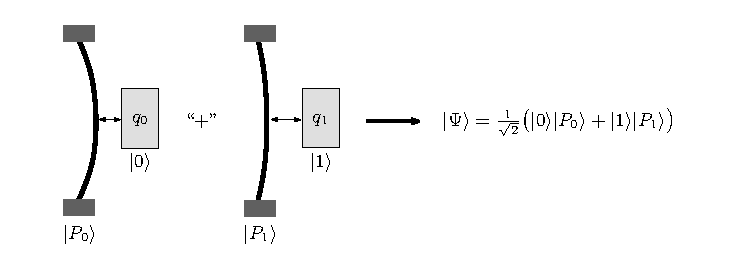
\includegraphics[width=.96\linewidth]{figures/ch06_fig27.pdf}
\caption{Armour、Blencowe、Schwab\cite{ref312}が提案した、ナノ機械共振器の二つの異なる位置の重ね合わせを生成する方法。箱の超伝導島の異なる電荷$q_0$、$q_1$に対応する基底状態$|0\rangle$、$|1\rangle$で記述されるCooper対箱を、共振器へ静電結合する。箱をコヒーレント重ね合わせ$(|0\rangle+|1\rangle)/\sqrt2$に準備し、適切な制御パルス列を加えると、もつれた箱・共振器の重ね合わせ$(|0\rangle|P_0\rangle+|1\rangle|P_1\rangle)/\sqrt2$が得られる。$|P_0\rangle$、$|P_1\rangle$は、共振器の識別できる二つの重心位置に対応する。}
\end{figure}

\subsubsectionlink*{QEMSにおけるデコヒーレンス}
上述の生成法の実用的な実現可能性を評価するには、その重ね合わせに影響するデコヒーレンスの主な源を理解することが重要である。まず、Cooper対箱自体も、もちろんデコヒーレンスを受ける。しかし、6.3.4節で述べたように、$\mu\mathrm s$領域の比較的長い時間は実験的に達成可能である\cite{ref289}。したがって、共振器自体の環境相互作用によるデコヒーレンスに焦点を当てられる。

興味深いことに、現在の実験的証拠\cite{ref318,ref319}、および初期の結果（たとえば\cite{ref320,ref321}）は、QEMSの主な散逸源、したがってデコヒーレンス源も、共振器の最低の基本曲げモードと、共振器内の局在した欠陥との相互作用かもしれないことを示す。これらの欠陥は有効二準位系で、電荷トラップ、不純物原子、弾性中心、共振器表面の結晶構造の乱れによる未結合手など、さまざまな物理的実現を取る。

現時点では、欠陥の基礎にある正確な物理的詳細や、曲げモードとの相互作用は、実験でも理論でも、まだ十分理解されていない。上述の空間的重ね合わせはまだ実現されていないため、QEMSのデコヒーレンスの直接実験データは存在しない。しかし、近年の実験は、散逸の特徴的性質について、貴重な情報を与えた\cite{ref318,ref319}。

散逸には一般にデコヒーレンスが伴うが、その逆は成り立たないので、こうした測定から、デコヒーレンスの性質についても知見を得られる。たとえば散逸データから、欠陥で構成される環境の有効スペクトル密度を取り出せるかもしれない。共振器と欠陥の相互作用の適切な模型があれば、それを使って、関係するデコヒーレンス係数と動力学を計算できる。そして、上述の重ね合わせの特徴的デコヒーレンス率を評価し、生成法の実現可能性を検討できる。ゆえに、QEMSの散逸とデコヒーレンスの現実的模型の開発が、主要な目標の一つとなる\cite{ref242,ref314,ref315}。それは理論的理解を高めるだけでなく、重ね合わせの実験的実現を前進させ、QEMSの実装全般の改善も示唆する。

% 原文 p.288
\hypertarget{srcpage:288}{}\label{srcpage:288}
Armour、Blencowe、Schwabは、最初の提案\cite{ref312}で、5.2節のよく研究された量子Brown運動模型を用い、空間的な箱・共振器重ね合わせ(6.37)のデコヒーレンス時間を評価した。中心調和振動子が基本曲げモードを表し、ほかの調和振動子からなる環境へ弱く結合する。しかし上述のように、mK温度のナノ機械共振器の環境は、欠陥を表す二準位系の集まりとして記述する方が、より現実的かもしれない。これらを量子スピン$1/2$粒子として模型化すれば、振動子・スピン模型が得られる。その弱結合マスター方程式は、5.4.2節で導いた［(5.198)参照］。

しかし、この模型の減衰率の温度依存性［(5.200)参照］は、散逸率が温度とともに増加するというQEMSの実験データ\cite{ref318,ref319}と一致しない。この不一致は、欠陥の少なくとも一部を、さらに別の、デコヒーレンスと散逸を生む環境に強く結合した、スピン$1/2$粒子として扱うべきことを示す（図6.28）。この環境は、スピンのトンネルを非コヒーレントにし、緩和も生じさせ、古典的二準位揺動子に似た欠陥動力学を誘起する。スピン浴から過剰エネルギーを吸収することで、その飽和を防ぐ。したがって、より現実的な模型は、独立なスピン・ボソン模型、すなわち振動子浴と相互作用するスピンを複数個、中心調和振動子へ結合したものかもしれない。この模型の最初の研究は、ごく最近行われた\cite{ref242}。このようにQEMSは、異なるデコヒーレンス・散逸模型を、実験で区別し検証する機会を与える。
\begin{figure}[htbp]\centering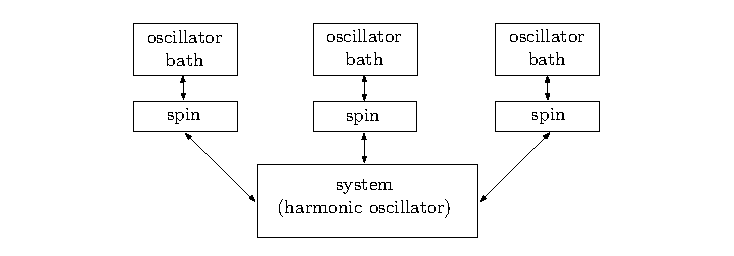
\includegraphics[width=.86\linewidth]{figures/ch06_fig28.pdf}
\caption{QEMSのデコヒーレンスと散逸の、考えられる模型。中心系は、ナノ機械共振器の基本曲げモードを表す調和振動子からなる。これは、スピン$1/2$粒子として模型化した二準位欠陥の集合と相互作用する。さらに各スピンは、散逸的な振動子浴へ結合し、その浴が、そうしなければ容易に飽和するスピン環境から、エネルギーを吸収する。}
\end{figure}

% 原文 p.289
\hypertarget{srcpage:289}{}\label{srcpage:289}
\subsectionlink{展望}
Schrödingerが1935年に猫の逆説を初めて描いたとき、それを純粋な思考実験、経験する巨視的世界へ量子力学を適用したときに生じる、明らかに「不合理な」帰結の例と考えた。しかし、過去数年、比較的小さいとはいえ、それでも巨視的なSchrödingerの猫を、実験室で育て、観測することに、大きな進展があった。本章では、数十個の光子を含む、巨視的に区別できる二状態の重ね合わせの生成（6.1節）、重い$\mathrm C_{70}$分子の干渉模様の観測（6.2節）、逆方向に流れる二つの$\mu\mathrm A$電流の重ね合わせの存在の検証（6.3節）を達成した実験を述べた。

各実験で研究者は、デコヒーレンスの漸進的作用、すなわち環境との相互作用により、重ね合わせがやがて観測できなくなる様子も、明示的に測定できた。こうして、量子から古典への移行の滑らかさを、明瞭に見た。量子状態を古典状態へ不連続に変換するような、固定された障壁は、量子領域と古典領域の間にない。系と環境の相互作用を操作することで、移行の動力学と時間尺度を直接変えられる。

したがって、本章の実験は、デコヒーレンスの範囲が、周囲の巨視的物体の、実効的に瞬時の「局在化」を指すだけよりも、はるかに広いことを示す。デコヒーレンスは、実効的古典性の出現を、漸進的で制御可能な過程として説明する。それは実験室で直接観測・検証でき、標準的量子力学の形式で厳密に理論記述できる。

ここでは、理論と実験の相互作用が非常に密接である。デコヒーレンス時間尺度や、その動力学のほかの性質の測定によって、模型を実験室で直接試せる。そして、模型がどの程度現実的で、物理的に適切かを学ぶ。一方、模型は、既存と将来の実験について貴重な情報を与える。ある配置で、どの段階の「巨視性」で量子から古典への移行を予想すべきか、あるパラメーターの組でどの種の「Schrödingerの子猫」を生成・観測できそうか、さらに「猫らしい」重ね合わせを作るため、実験をどう改善できるかを教える。本章では、理論的方式で提案された特定の重ね合わせの生成を、まだ達成していない二領域、Bose--Einstein凝縮（6.4.1節）と量子電気機械系（6.4.2節）を述べた。それでも、測定データとデコヒーレンス模型を組み合わせれば、望ましい重ね合わせを「見る」のを妨げる、物理的に関係する機構を同定でき、
% 原文 p.290
\hypertarget{srcpage:290}{}\label{srcpage:290}
有害な効果を弱める方法が示唆される。

自然に生じる問いは、巨視的に異なる状態の重ね合わせの実験が、将来どこへ向かうのか、その結果が量子力学の理解や、量子コンピューターなどの大規模量子系の構築に、どのような含意を持つか、ということである。答えは多いので、主要な点を少しだけ挙げよう。

まず、これまで調べた尺度では、既存の実験的証拠は、重ね合わせ原理の根本的限界を示していない。環境との望ましくない相互作用を最小にする適切な設計で、デコヒーレンスを十分制御できる限り、その限界は精密な定量解析が可能だが、「古典的」状態のどのような数の重ね合わせも、生成・観測できるように見える。

したがって、今後数年、巨視的に異なる状態の重ね合わせの、達成可能な「大きさ」の限界を、さらに押し進める多くの実験を見ることになる、といってよい。近いうちに、ウイルスのような、さらに大きい生体分子の干渉模様を観測し、凝縮体やナノ機械共振器の重ね合わせを実現し、超伝導量子ビットのデコヒーレンス時間を飛躍的に延ばせるかもしれない。このような実験は、重ね合わせ原理が破れる可能性を探し続けることによっても動機づけられる。しかし、デコヒーレンスは局所観測者からは見かけの破れを生じさせるので、十分にそれを遮蔽しながら、ユニタリー発展からのずれを誘起する機構には適度に敏感な実験を設計するのは、今後も非常に難しいだろう（8.4節および\cite{ref286,ref322}参照）。

ますます異なる巨視的状態の重ね合わせを生成・観測できることは、その重ね合わせ自体や、デコヒーレンスと量子力学一般に関わる、根本的な解釈上の問いを解かないことを、強調する必要がある。量子状態（2.1節）、特に重ね合わせ状態（2.2.1節）の適切な解釈と物理的意味の問題は、2.2.2節のStern--Gerlach実験のような、微視的設定ですでに明らかである。近年の巨視的重ね合わせ実験は、Schrödingerの猫型の直観に反する色合いを加えるかもしれないが、解釈の根本問題を解きも、深めもしない。

特に、環境を含む全体の量子状態でコヒーレンスが持続することをどう理解するか、したがって、デコヒーレンスの密度行列記述から生じる量子状態の非真正混合を、基礎にある何らかの量子的実在へどう適切に関係づけるかは、基礎論上の論争であり続ける。
% 原文 p.291
\hypertarget{srcpage:291}{}\label{srcpage:291}
ここで論じた型の実験は、少なくとも「実在の本性」についての先入観へ、さらに挑むことで、議論を今後も明るく照らすだろう。純粋にユニタリーな動力学からのずれを、実験が決定的に示す、あるいは排除できるようになれば、量子力学と量子的実在の構造について、新たな知見を得るか、得ざるを得なくなるかもしれない。しかし現在は、本章の驚くべき実験的成果を踏まえても、解釈の問題は残り続ける。

